%--------------A VOTRE ATTENTION-------------%
% Les étudiants  qui disposent de plus de 3 chapitres dans leurs travaux peuvent en complèter
% Les Membres doivent figurer dans la dernière version finale du mémoire pour dépôt de mémoire

\documentclass{iid}
\usepackage{titletoc}
\setlength{\glsdescwidth}{0.65\textwidth}
% \usepackage{lscape}

\typeMemoire{Diplôme d’Ingénieur d'État }
\optionFormation{\textbf{Informatique et Ingénierie des Données}\\ 
\includegraphics[scale=0.08]{images/logoIID.png}}
\etudiant{Ziyad \textbf{RAKIB}}
\titreDuMemoire{Titre du mémoire} 
\dateSoutenance{15/06/2023}
%\promo{2\up{ème}}
\anneeScolaire{\the\year}


%%maitre de mémoire
\encadrants{Abdelghani \textbf{Ghazdali}\\Nidal \textbf{Lamghari}}

%% Membres du Jury
\jurys{%
\begin{tabular}{lll}
	Nom et prénoms du président &  Entité & Président \\
	Nom et prénoms de l'examinateur & Entité & Examinateur \\
	Nom et prénoms du rapporteur &  Entité & Rapporteur \\
		Nom et prénoms du rapporteur &  Entité & Rapporteur \\
\end{tabular}	
}


\hypersetup{
 pdftitle={--},
 pdfauthor={--},
 pdfsubject={--},
 pdfkeywords={--} 
 }

\color{bookColor}

%importation du glossaire
\loadglsentries{glossaire_reduit}

\begin{document}




\pageDeGarde%\pageTitre

\pagecolor{white}

%% page vide
\thispagestyle{empty}\ \clearpage
ehrig2006graph
\newpage
% sommaire
\pagenumbering{roman}

\setcounter{tocdepth}{0}
\startlist{toc}
\printlist{toc}{}{\chapter*{Sommaire}}
\setcounter{tocdepth}{5}

%% rdedicaces
\dedicace

\begin{fquote}
\begin{center}
\large{

\uppercase{à} mLorem ipsum dolor sit amet, consectetur adipiscing elit. Proin posuere euismod neque, non semper nibh viverra sed. Praesent ut varius magna. Fusce ipsum ante, semper nec interdum at, semper et lacus. Nulla ultrices magna a fringilla finibus,\\[12pt]
\uppercase{à} Lorem ipsum dolor sit amet, consectetur adipiscing elit. Proin posuere euismod neque, non semper nibh viverra sed. Praesent ut varius magna. Fusce ipsum ante, semper nec interdum at, semper et lacus. Nulla ultrices magna a fringilla finibus,\\[12pt]
\uppercase{à} Lorem ipsum dolor sit amet, consectetur adipiscing elit. Proin posuere euismod neque, non semper nibh viverra sed. Praesent ut varius magna. Fusce ipsum ante, semper nec interdum at, semper et lacus. Nulla ultrices magna a fringilla finibus,\\[12pt]
\uppercase{à} tous ceux qui me sont chers, à vous tous\\[12pt]
Merci.
}
\end{center}
\bigskip
\medskip
\end{fquote}

\begin{adjustwidth}{2cm}{1cm}
\hspace*{\fill} \textbf{\textit{\large{- Abdelghani}}}
\end{adjustwidth}

\clearpage

\newpage 

%% remerciements
\remerciements

Tout d’abord, je remercie le grand Dieu puissant de nous donné la puissance pour continuer et dépasser toutes les difficultés.

\medskip

J’adresse mes remerciements à, \textbf{\LR{\large{Monsieur Abdelghani Ghazdali}}}, chef de filière Informatique et Ingénierie des Données qui a su assurer le bon déroulement des séances d’encadrement du début à la fin.

\medskip

Je tiens également à adresser mes sincères remerciements à \textbf{\LR{\large{Professeur Nidal Lamghari}}}, pour ses précieux conseils, son expertise et sa disponibilité tout au long de cette expérience. Votre encadrement attentionné m'a permis d'approfondir mes connaissances et de progresser dans mes compétences techniques. Je suis reconnaissant d'avoir pu bénéficier de votre expertise et de votre soutien constant.

\medskip

Au terme de ce travail, je tiens également à exprimer mes sincères remerciements et ma gratitude envers tous ceux qui, par leur enseignement, par leur soutien et leurs conseils, ont contribué au déroulement de ce projet.

\medskip
Par ailleurs, je tiens à exprimer ma gratitude envers \textbf{\LR{\large{IZICAP}}}, où j'ai eu la chance de réaliser mon projet de fin d'études. Je suis reconnaissant envers toute l'équipe de \textbf{\LR{\large{IZICAP}}} pour m'avoir accueilli chaleureusement et pour m'avoir permis de mettre en pratique mes connaissances académiques dans un environnement professionnel. Votre expertise, votre mentorat et vos ressources ont été d'une valeur inestimable pour la réalisation de ce projet.

\medskip

Je tiens à remercier spécialement \textbf{\LR{\large{M. Bilal SLAYKI}}}, mon encadrant en entreprise, pour son soutien constant, ses orientations judicieuses et son accompagnement précieux tout au long de ce projet. Votre expérience, vos conseils éclairés et votre bienveillance m'ont inspiré et ont grandement contribué à ma croissance professionnelle. Je vous suis reconnaissant d'avoir partagé votre expertise avec moi et d'avoir été un mentor exceptionnel.

\medskip

Finalement, mes remerciements s’adressent aussi à l’ensemble du corps professoral et administratif de l’ENSA Khouribga pour l’effort qu’ils fournissent afin de nous garantir une bonne formation et à l’équipe administrative et technique pour tous les services offerts.
\newpage 

% Résume
\resume
%\selectlanguage{french}






Ce rapport fournit une analyse approfondie du projet complexe entrepris pour faire évoluer la source de données de Izicap. Le projet a nécessité la suppression de MariaDB et la mise en place de Delta Lake, une solution de stockage et de traitement de données hautes performances. De plus, l'architecture monolithique existante a été divisée en microservices utilisant Spring Boot comme backend avec un connecteur approprié pour Delta Lake, et les micro-frontends ReactJS comme frontend.

\medskip

Le projet présentait de nombreux défis qui nécessitaient l'application de technologies et de stratégies avancées. Celles-ci comprenaient la migration des données, la garantie de la cohérence et de l'exactitude des données, la gestion de la complexité des systèmes distribués et l'intégration de diverses technologies et services. Le rapport décrit les différentes solutions développées pour relever ces défis, notamment l'utilisation d'algorithmes de traitement de données avancés, d'architectures informatiques distribuées et de la conteneurisation.

\medskip

Malgré les défis rencontrés, le projet reste un travail en cours. Le rapport donne un aperçu des efforts en cours pour améliorer l'évolutivité, les performances et la fonctionnalité globale du projet.

\vspace{1cm}


\noindent\rule[2pt]{\textwidth}{0.5pt}

{\textbf{Mots clés :}}
Projet, Source de données, Delta Lake, Monolith, Microservice, Spring Boot, ReactJS, Micro-Frontend, Back-End, Front-End, Données, Évolutivité, Performance.
\\
\noindent\rule[2pt]{\textwidth}{0.5pt}

\clearpage


\newpage

% Résume
\resumeAn
%\begin{abstract}
This final year project report highlights the different stages of our project to transform a Groovy-based monolithic architecture into a Java-based microservices architecture, while transitioning from AngularJS to React and adopting a microfrontend approach. Our goal was to enhance the flexibility, maintainability, performance, data consistency, and modularity of our application.
\medskip

Initially, our codebase was developed as a monolith using Groovy. The first step of our project involved analyzing the monolithic architecture and identifying components that could be isolated into independent microservices. Concurrently, we evaluated the benefits of migrating from the outdated AngularJS framework to the more modern and performant React framework.

\medskip
We proceeded with the design and implementation of these microservices using Spring Boot, ensuring loose coupling between functionalities and effective communication among services. Simultaneously, we gradually migrated our AngularJS code to React, rewriting existing features according to React's best development practices.  
\medskip

To ensure data consistency among microservices, we implemented Delta Lake, an incremental data management technology. Delta Lake guaranteed reliable data and simplified secure read and write operations between services. Java connectors facilitated communication between the React-based frontend and Delta Lake, ensuring robust and secure connectivity. These connectors also enabled efficient read and write operations, ensuring data integrity and consistency.

\medskip
In parallel, we adopted a microfrontend approach for our frontend architecture, decoupling frontend features into autonomous modules. This provided greater flexibility and the ability to develop and deploy modules independently.

\medskip

Finally, to facilitate deployment and management of our microservices, React, and microfrontend architecture, we adopted Kubernetes and Docker. These tools enabled efficient orchestration, scaling of services, and simplified deployment across different environments.
\medskip

In conclusion, our project resulted in significant improvements in flexibility, maintainability, performance, data consistency, and modularity of our application. The transition from a Groovy-based monolithic architecture to a Java-based microservices architecture, combined with the migration from AngularJS to React, the adoption of Delta Lake, Java connectors, microfrontend, Kubernetes, and Docker, collectively optimized our system.

    \noindent\rule[2pt]{\textwidth}{0.5pt}
    {\textbf{Mots-clés :}}
    Monolithique, Groovy, Microservices, AngularJS, React, Delta Lake, Microfrontend, Kubernetes, Docker\\
    \noindent\rule[2pt]{\textwidth}{0.5pt}
\clearpage
\newpage

% Résume
%\resumeAr
\setcode{utf8}

\chapter*{\hfill \RL{ملخص}}




\setstretch{1.3}
\begin{flushright}
\RL{
 في هذا التقرير، وردت إشارة إلى تنفيذ نظام كشف الوجه. والهدف من ذلك هو الكشف عن وجوه الناس المهتمين في منشور
  معين.
لقد إستعملنا لهذا الغرض لوحة الكترونية \LR{Raspberry pi 2} بالإضافة إلى وحدة الكاميرا الخاصة بها لملاحقة الوجوه و العين.
يستخدم  تطبيق كشف الوجه  خوارزمية قوية  لفيولا جونز مع  تدريب المصنف للكشف عن الوجه الإنساني والعينين، عن طريق اختيار أفضل مصنف ممكن.
سيتم حفظ البيانات لكل إعلان في قاعدة بيانات \LR{MySQL} . وقد تم إنشاء تطبيق ويب لهذا الغرض والذي سيمكن المستخدم من   
معرفة عدد الأشخاص  والمدة الإجمالية للمشاهدة في الفترة (ساعة، يوم، شهر )  على شكل رسم بياني.
}
\end{flushright}


\vspace{1cm}


\noindent\rule[2pt]{\textwidth}{0.5pt}
\begin{flushright}
\RL{\textbf{
كلمات مفتاحية \LR{:} } ك ك  
}

\end{flushright}
\noindent\rule[2pt]{\textwidth}{0.5pt}

%\end{abstract}







\newpage

\selectlanguage{french}
\dominitoc% initializer les minitoc
\tableofcontents
\newpage

%liste des figures
\listoffigures 
\newpage

%liste des tableaux
\listoftables
\newpage

%%liste des algo
%\listofalgorithmes
%\newpage
%


%% Les sigles et acronymes
\listofsigle\begin{tabular}{rl}
API & Application programming interface \\
VSC & Visual Studio Code \\
DL & Delta Lake \\
REST & RepresEntational State Transfer \\
AWS & Amazon Web Services \\
GCP & Google Cloud Platform \\
AZR & Microsoft Azure \\
S3 & Simple Storage Service \\
IAM & Identity and Access Management \\
MinIO & Minimal Object Storage \\
SQL & Structured Query Language \\
DB & Database \\
ACID & Atomicity, Consistency, Isolation, Durability \\
OLTP & Online Transaction Processing \\
OLAP & Online Analytical Processing \\
ReactJS & React JavaScript \\
SPA & Single Page Application \\
JS & JavaScript \\
CSS & Cascading Style Sheets \\
HTML & Hypertext Markup Language \\
UI & User Interface \\
API & Application Programming Interface \\
Spark & Apache Spark \\
Hadoop & Apache Hadoop \\
HDFS & Hadoop Distributed File System \\
YARN & Yet Another Resource Negotiator \\
MapReduce & MapReduce Programming Model \\
Metadata & Data about Data \\
ETL & Extract, Transform, Load \\
ELT & Extract, Load, Transform \\
CRM & Customer Relationship Management \\
RDBMS & Relational Database Management System \\

\end{tabular}

\newpage

%% Les sigles et acronymes
%\setglossarystyle{altlist}
%\printglossary[title=Liste des acronymes, toctitle=Liste des acronymes, type=\acronymtype]
%\newpage

% Le glossaire proprement dit
%\setglossarystyle{super}
%\printglossary[type=main]


\pagenumbering{arabic}
\setcounter{page}{1}
%%introduction
\introduction
bla bla bla \gls{acro} puis \Gls{acroglo} et enfin \gls{glossaire}
%\lhead[]{} \rhead[]{} \chead[]{}
\selectlanguage{french}
\fancyhead[L]{\tiny \leftmark}
\fancyhead[R]{\scriptsize \rightmark}
\fancyfoot[C]{\thepage}

\chapter{fknznefkljebngflkjen}\label{chap:1}
\minitoc
\addcontentsline{toc}{section}{Introduction}
\section*{Introduction}

\section{About}
Izicap est un pionnier dans l'utilisation des données de cartes de paiement et les transforme en une connaissance client et des informations commerciales puissantes pour les commerçants, leur permettant de gérer leurs propres programmes de fidélité et campagnes de marketing numérique. 
Ces services marketing, fournis par les acquéreurs utilisant les solutions SaaS d'Izicap, redonnent rapidement de la croissance aux entreprises marchandes en renforçant les dépenses et la fidélité de leurs clients (les titulaires de carte). 
La solution innovante de CRM et de fidélité liée aux cartes d'Izicap donne aux acquéreurs un avantage concurrentiel en monétisant leurs données de transactions de paiement, en générant de nouvelles sources de revenus et en améliorant leurs capacités de rétention.
Après s'être solidement implanté en France grâce à des partenariats avec le Groupe BPCE et le Crédit Agricole, Izicap s'est associé à Nexi, le premier acquéreur et Fintech en Italie et a rejoint le programme StartPath de Mastercard dans le but d'étendre considérablement sa portée mondiale. 
Izicap s'associe aux principaux fournisseurs de solutions de paiement tels qu'Ingenico, Verifone, Poynt et PAX, et rend sa solution CRM et Fidélité liée à la carte disponible sur les terminaux de paiement les plus populaires et les plus innovantes.

\section{Organigramme}
informations sur Izicap

\addcontentsline{toc}{section}{Conclusion}
\section*{Conclusion}

 
 \chapter{Delta Lake}\label{chap:2}
 \addcontentsline{toc}{section}{Introduction}

\section*{Introduction}

L'informatique décisionnelle, également connue sous le terme de Business Intelligence (BI), englobe les processus, les technologies et les outils utilisés pour collecter, stocker, analyser et présenter les données dans le but de soutenir la prise de décision et d'aider les entreprises à obtenir des informations exploitables. L'informatique décisionnelle implique la transformation des données brutes en informations significatives et en connaissances exploitables pour les décideurs. On va voir dans ce chaptire pourquoi on a decidé d'opter pour Delta Lake au lieu de ses contre-parts.

\section{Différence entre un data warehouse, un data lake, un datalakehouse et un delta lake}
\begin{enumerate}
    \item[$\bullet$] \textbf{Data Warehouse:} Un data warehouse est une base de données centralisée qui est spécifiquement conçue pour le reporting et l'analyse. Il stocke les données structurées provenant de différentes sources, les organise selon un modèle de données prédéfini et les optimise pour des requêtes analytiques. Les données dans un data warehouse sont généralement cohérentes, intégrées et historisées. Cependant, la construction et la maintenance d'un data warehouse peuvent être complexes et coûteuses.
    \item[$\bullet$] \textbf{Data Lake:} Un data lake est un référentiel de données centralisé qui stocke de grandes quantités de données brutes, structurées et non structurées. Contrairement au data warehouse, le data lake ne nécessite pas une modélisation préalable des données. Il offre une grande flexibilité et évolutivité pour stocker des données hétérogènes. Cependant, l'intégration et la qualité des données peuvent être des défis dans un data lake.
    \item[$\bullet$] \textbf{Datalakehouse:} Le datalakehouse est une architecture émergente qui combine les avantages du data warehouse et du data lake. Il permet de stocker et de traiter à la fois des données brutes et des données structurées dans un environnement centralisé. Cette approche hybride offre la flexibilité d'un data lake et la capacité d'analyse d'un data warehouse. Cependant, la mise en place d'un datalakehouse peut nécessiter des efforts supplémentaires pour garantir la qualité des données et l'efficacité des requêtes.
    \item[$\bullet$] \textbf{Delta Lake:} Delta Lake est une technologie qui s'intègre aux data lakes existants pour fournir des fonctionnalités supplémentaires, telles que la gestion des transactions ACID (Atomicité, Cohérence, Isolation, Durabilité), la gestion des mises à jour incrémentielles et la garantie de la cohérence des données. Delta Lake est construit sur Apache Parquet et Apache Arrow, ce qui permet d'accélérer les requêtes analytiques et d'améliorer les performances globales. Cependant, l'utilisation de Delta Lake peut nécessiter des compétences techniques supplémentaires et peut avoir un impact sur la complexité de l'architecture de données. 
\end{enumerate}

% \subsection{Avantages et inconvénients de chaque architecture}

\subsection{Data Warehouse}
\textbf{Avanatges:}
\begin{enumerate}
    \item Données cohérentes et intégrées
    \item Modélisation préalable des données pour une analyse optimisée
    \item Hautes performances pour les requêtes analytiques
\end{enumerate}

\textbf{Inconvénients:}
\begin{enumerate}
    \item Coût élevé de construction et de maintenance
    \item Complexité de la modélisation des données
    \item Limitations pour l'intégration de données non structurées
\end{enumerate}

\subsection{Data Lake}
\textbf{Avanatges:}
\begin{enumerate}
    \item Stockage économique de grandes quantités de données
    \item Flexibilité pour intégrer des données brutes et non structurées
    \item Capacité à traiter des données de différentes sources
\end{enumerate}

\textbf{Inconvénients:}
\begin{enumerate}
    \item Difficulté à maintenir la qualité des données et la gouvernance
    \item Besoin d'outils avancés pour l'analyse et le traitement des données
    \item Requiert des compétences techniques pour l'exploitation efficace des données
\end{enumerate}

\subsection{Datalakehouse}
\textbf{Avanatges:}
\begin{enumerate}
    \item Combinaison des avantages du data warehouse et du data lake
    \item Flexibilité pour stocker et analyser des données brutes et structurées
    \item Possibilité d'évoluer en fonction des besoins évolutifs
\end{enumerate}

\textbf{Inconvénients:}
\begin{enumerate}
    \item Nécessite des efforts supplémentaires pour la qualité des données
    \item Complexité accrue de l'architecture de données
    \item Besoin de compétences techniques pour la mise en place et la gestion
\end{enumerate}

\subsection{Delta Lake (Datalakehouse)}
\textbf{Avanatges:}
\begin{enumerate}
    \item Gestion des transactions ACID pour une cohérence des données
    \item Prise en charge des mises à jour incrémentielles et du traitement des flux de données
    \item Hautes performances pour les requêtes analytiques
\end{enumerate}

\textbf{Inconvénients:}
\begin{enumerate}
    \item Nécessite des compétences techniques spécifiques
    \item Impact sur la complexité de l'architecture de données existante
    \item Peut nécessiter des adaptations pour une intégration transparente avec les outils existants
\end{enumerate}

\begin{figure}[H]
\centering
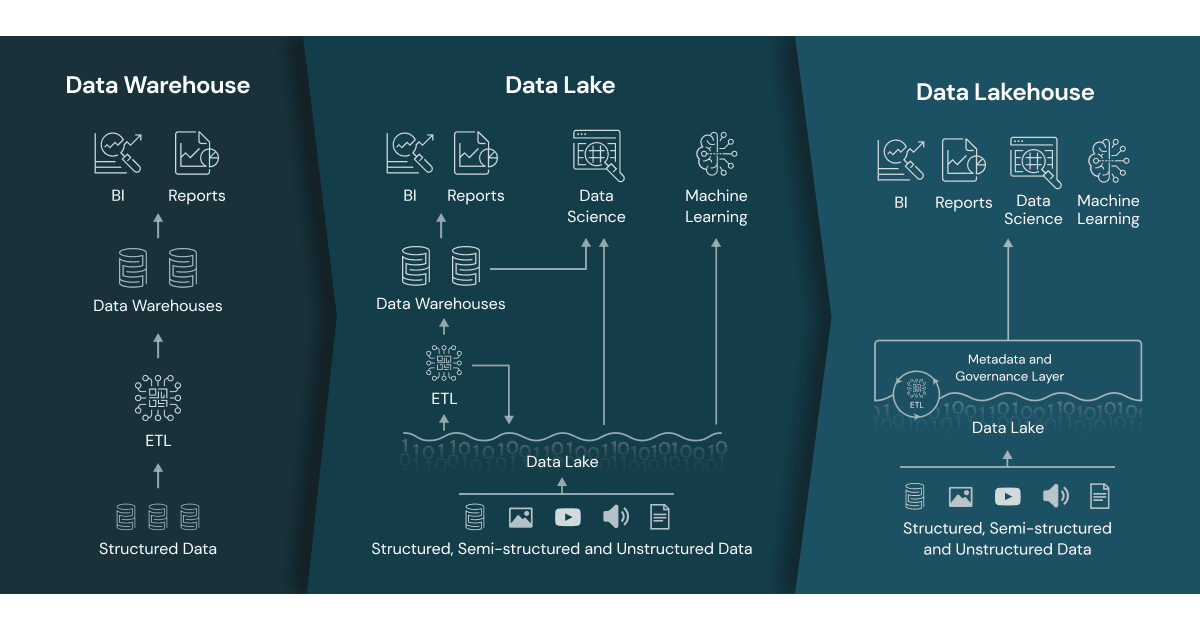
\includegraphics[width=\linewidth]{images/data-warehouse-data-lake-datalakehouse.png}
\caption{Data Warehouse vs Data Lake vs Data Lakehouse}\label{fig:data-warehouse-data-lake-datalakehouse}
\end{figure}

\section{Différence entre une architecture microservices et une architecture monolithique}
\begin{enumerate}
    \item[$\bullet$] \textbf{Monolithe:} un monolithe est une application qui est conçue comme une entité unique et indivisible. Toutes les fonctionnalités de l'application sont regroupées dans un seul code base, partageant les mêmes ressources, bases de données et déploiements. Dans une architecture monolithique, il n'y a pas de découpage clair des fonctionnalités en services indépendants. Toute modification ou évolution de l'application nécessite des changements au niveau global.
    \item[$\bullet$] \textbf{Microservice:} Un microservice est une approche architecturale dans laquelle une application est construite comme un ensemble de services indépendants et autonomes, chacun se concentrant sur une fonction spécifique de l'application. Chaque microservice est développé, déployé et géré de manière indépendante, ce qui permet une évolutivité, une flexibilité et une maintenance plus faciles. Les microservices communiquent entre eux via des interfaces bien définies, généralement basées sur des API REST ou des messages.
\end{enumerate}

\subsection{Avantages et Inconvénients de l'architecture monolithique}
\textbf{Avanatges:}
\begin{enumerate}
    \item \textbf{Simplicité de développement initial :} L'approche monolithique permet de développer rapidement une application en regroupant toutes les fonctionnalités dans un seul code base. Cela facilite la gestion des dépendances et la coordination des différentes parties de l'application.
    \item \textbf{Moins de complexité opérationnelle :} Avec une architecture monolithique, il y a moins de composants et de services à gérer, ce qui simplifie les opérations de déploiement, de surveillance et de gestion. Tout est regroupé au sein d'un seul déploiement, ce qui peut être plus facile à gérer pour les équipes opérationnelles.
    \item \textbf{Communications internes plus rapides :} Dans une architecture monolithique, les communications entre les différentes parties de l'application sont plus rapides car elles se font généralement via des appels de méthode internes. Cela peut être bénéfique en termes de performances et de latence réduite.
\end{enumerate}

\textbf{Inconvénients:}
\begin{enumerate}
    \item \textbf{Difficulté à faire évoluer et à maintenir:} Avec une architecture monolithique, les évolutions et les mises à jour peuvent être plus complexes, car chaque changement doit être effectué sur l'ensemble de l'application. Cela peut rendre le processus de développement plus lent et entraîner des risques d'erreurs lors des déploiements.
    \item \textbf{Rigidité technologique:} Une architecture monolithique peut entraîner une rigidité technologique, car toutes les parties de l'application doivent utiliser les mêmes technologies et langages de programmation. Cela peut limiter les possibilités d'adopter de nouvelles technologies ou de faire évoluer des parties spécifiques de l'application de manière indépendante.
    \item \textbf{Difficulté à isoler les problèmes:} En cas de problème ou de bug, il peut être plus difficile de les isoler et de les résoudre dans une architecture monolithique. Étant donné que toutes les fonctionnalités sont regroupées dans un seul code base, il peut être complexe de localiser l'origine exacte du problème.
    \item \textbf{Moins de flexibilité en termes d'évolutivité:} L'architecture monolithique peut poser des défis en termes d'évolutivité. Si une partie de l'application nécessite plus de ressources pour gérer une charge élevée, il peut être difficile d'ajuster cette partie spécifique sans augmenter les ressources globales de l'application.
\end{enumerate}

\subsection{Avantages et Inconvénients de l'architecture microservices}
\textbf{Avanatges:}
\begin{enumerate}
    \item \textbf{Scalabilité et évolutivité:} Les microservices permettent de découper l'application en plusieurs services autonomes et indépendants, ce qui facilite la scalabilité horizontale. Chaque microservice peut être déployé, mis à l'échelle et mis à jour indépendamment, ce qui permet de gérer efficacement les variations de charge et de garantir une évolutivité facile en fonction des besoins de l'entreprise.
    \item \textbf{Flexibilité technologique:} Les microservices offrent la possibilité d'utiliser différentes technologies et langages de programmation pour chaque service. Dans notre cas, l'utilisation de Spring Boot nous permet de profiter de son écosystème riche et de ses fonctionnalités avancées pour le développement rapide d'applications. Cela permet également d'adopter des technologies spécifiques en fonction des besoins de chaque microservice, favorisant ainsi la flexibilité technologique.
    \item \textbf{Indépendance et autonomie:} Chaque microservice est conçu pour fonctionner de manière autonome, ce qui permet une meilleure isolation des fonctionnalités et des responsabilités. Cela facilite la maintenance, le test et le déploiement des services de manière indépendante, réduisant ainsi les risques d'impact sur l'ensemble du système en cas de modifications ou de problèmes.
    \item \textbf{Développement et déploiement rapides:} Les microservices permettent une approche de développement agile en favorisant des cycles de développement plus courts. Les équipes peuvent se concentrer sur des fonctionnalités spécifiques et les développer de manière indépendante, ce qui accélère le développement global du système. De plus, les microservices peuvent être déployés de manière continue grâce à l'utilisation de techniques de déploiement automatisées, facilitant ainsi les mises à jour fréquentes et rapides.
    \item \textbf{Facilité de maintenance et de débogage:} En raison de leur nature modulaire, les microservices facilitent la maintenance et le débogage du système. En cas de problème ou d'erreur, il est plus facile d'identifier le service spécifique concerné et de résoudre le problème sans impacter l'ensemble du système.
\end{enumerate}

\textbf{Inconvénients:}
\begin{enumerate}
    \item \textbf{Complexité de la gestion des communications:} Les microservices impliquent une communication entre différents services, généralement via des API REST ou des messages. La gestion de ces communications peut devenir complexe, en particulier lorsque de nombreux services sont impliqués. Des problèmes tels que la latence, la cohérence des données et la gestion des erreurs peuvent se poser.
    \item \textbf{Surcharge de développement initial:} Le développement de microservices nécessite un effort supplémentaire pour découper correctement les fonctionnalités, définir les interfaces et mettre en place une infrastructure appropriée pour le déploiement et la communication des services. Cela peut augmenter la charge de travail initiale et nécessiter des compétences spécifiques en matière d'architecture distribuée.
    \item \textbf{Gestion de la cohérence des données:} Avec des microservices, chaque service peut avoir sa propre base de données ou son propre stockage de données. Cela peut rendre la gestion de la cohérence des données plus complexe, en particulier lorsqu'il y a des mises à jour simultanées impliquant plusieurs services. Des techniques telles que les transactions distribuées ou les événements asynchrones peuvent être nécessaires pour maintenir la cohérence des données.
    \item \textbf{Déploiement et gestion de plusieurs services:} Avec les microservices, il y a un nombre accru de services à déployer, gérer et surveiller. Cela peut nécessiter des compétences supplémentaires en matière d'automatisation des déploiements, de gestion des conteneurs ou de gestion des clusters. Le suivi des performances et du comportement de chaque service peut également devenir plus complexe.
    \item \textbf{Coût de l'infrastructure:} Les microservices peuvent nécessiter une infrastructure plus complexe et des ressources supplémentaires pour fonctionner efficacement. Chaque service doit être déployé et exécuté indépendamment, ce qui peut entraîner une augmentation des coûts liés aux ressources informatiques et à la gestion de l'infrastructure.
\end{enumerate}

\begin{figure}[H]
\centering
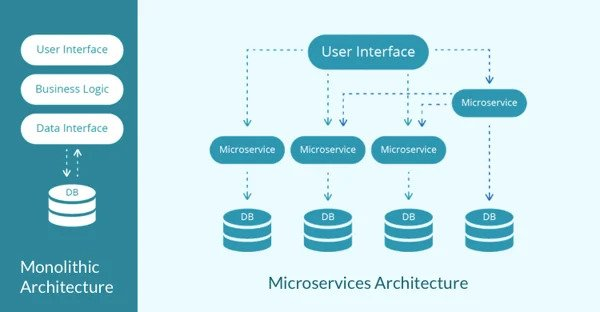
\includegraphics[width=0.6\linewidth]{images/monolithicvsmicroservice.jpg}
\caption{Architecture monolithique vs microservice}\label{fig:monolithevsmicroservice}
\end{figure}

\section{Différence entre une architecture microfrontends et une architecture monolithique fronend}
\begin{enumerate}
    \item[$\bullet$] \textbf{Monolithe frontend:} Un frontend monolithique est une approche architecturale où l'application frontend est développée comme une seule entité, généralement en utilisant un framework spécifique tel qu'AngularJS. Toutes les fonctionnalités, les vues et les logiques de l'interface utilisateur sont regroupées dans un seul code base.
    \item[$\bullet$] \textbf{Microfrontends:} Les microfrontends sont une approche architecturale où une application frontend est divisée en plusieurs micro-applications indépendantes, chacune étant responsable d'une partie spécifique de l'interface utilisateur. Chaque micro-application peut être développée, déployée et évoluée de manière autonome, utilisant différents frameworks, langages et technologies.
\end{enumerate}

\subsection{Avantages et Inconvénients du monolithe frontend}
\textbf{Avanatges:}
\begin{enumerate}
    \item \textbf{Simplicité de développement initial:} L'architecture monolithique avec AngularJS offre une approche simple pour le développement initial de l'application frontend. Toutes les fonctionnalités sont regroupées dans un seul code base, ce qui facilite la coordination et la gestion du développement.
    \item \textbf{Facilité de communication entre les composants:} Dans une architecture monolithique, les composants AngularJS peuvent communiquer entre eux facilement via le système de directives et de services d'AngularJS. Cela permet une communication rapide et efficace entre les différentes parties de l'application. 
    \item \textbf{Interopérabilité des fonctionnalités:} Étant donné que toutes les fonctionnalités sont développées en utilisant AngularJS, il est plus facile de partager des fonctionnalités et des modules entre les différentes parties de l'application. Cela favorise la réutilisation du code et simplifie la maintenance.
\end{enumerate}

\textbf{Inconvénients:}
\begin{enumerate}
    \item \textbf{Difficulté à maintenir et à faire évoluer:} À mesure que l'application frontend devient plus complexe, la maintenance et l'évolution de l'architecture monolithique avec AngularJS peuvent devenir difficiles. Les modifications apportées à une partie de l'application peuvent avoir des répercussions sur l'ensemble du code base, ce qui rend le processus de développement plus lent et risqué.
    \item \textbf{Limitations de performance:} Dans une architecture monolithique, toutes les fonctionnalités sont chargées en même temps, ce qui peut entraîner des problèmes de performance si l'application devient volumineuse. Les temps de chargement peuvent être plus longs et l'application peut être moins réactive pour l'utilisateur.
    \item \textbf{Flexibilité limitée:} L'architecture monolithique avec AngularJS peut limiter la flexibilité technologique. Étant donné que toutes les parties de l'application sont développées en utilisant AngularJS, il peut être difficile d'introduire de nouvelles technologies ou de faire évoluer certaines parties spécifiques de l'application de manière indépendante.
\end{enumerate}

\subsection{Avantages et Inconvénients de l'architecture microfrontends}
\textbf{Avanatges:}
\begin{enumerate}
    \item \textbf{Indépendance des équipes de développement:} Chaque micro-application peut être développée par une équipe distincte, ce qui favorise une plus grande autonomie et une meilleure collaboration entre les équipes de développement. Chaque équipe peut choisir les technologies qui conviennent le mieux à ses besoins.
    \item \textbf{Évolutivité et facilité de maintenance:} L'architecture microfrontends permet de faire évoluer et de maintenir les différentes parties de l'application de manière indépendante. Les modifications apportées à une micro-application n'ont pas d'impact sur les autres, ce qui facilite la maintenance et permet de déployer rapidement de nouvelles fonctionnalités.
    \item \textbf{Flexibilité technologique:} Chaque micro-application peut utiliser la technologie, le framework ou le langage de programmation qui convient le mieux à son domaine spécifique. Cela permet d'introduire de nouvelles technologies et d'exploiter les avantages des derniers développements dans le domaine de l'ingénierie logicielle.
\end{enumerate}

\textbf{Inconvénients:}
\begin{enumerate}
    \item \textbf{Complexité accrue:} L'architecture microfrontends introduit une certaine complexité dans le développement et le déploiement de l'application. La gestion des interactions et de la communication entre les différentes micro-applications peut nécessiter une planification et une coordination supplémentaires.
    \item \textbf{Coût de développement initial:} Le développement d'une architecture microfrontends peut nécessiter un investissement initial plus important en termes de ressources et de temps. Le développement de plusieurs micro-applications distinctes et la mise en place de l'infrastructure nécessaire peuvent être plus coûteux que le développement d'une application monolithique.
    \item \textbf{Surcharge réseau:} L'utilisation d'une architecture microfrontends peut entraîner une surcharge réseau plus importante, car chaque micro-application nécessite des requêtes et des chargements de ressources distincts. Cela peut avoir un impact sur les performances de l'application et nécessiter une gestion efficace du réseau.
\end{enumerate}

\begin{figure}[H]
\centering
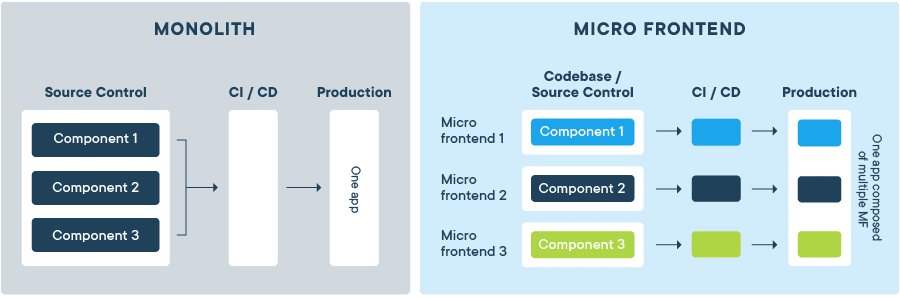
\includegraphics[width=\linewidth]{images/micro-frontend-vs-monolith-frontend.png}
\caption{Architecture monolithique frontend vs microfrontends}\label{fig:monolithfrontendvsmicrofrontends}
\end{figure}

\section{Cheminement de la solution}
\subsection{Partie Data}
Dans le cadre de notre solution, nous avons opté de remplacer l'exporter worker existant et les bases de données MariaDB par de remplacer l'exporter worker existant et les bases de données MariaDB par l'utilisation d'une architecture de type datalakehouse. Une datalakehouse est une approche hybride qui combine les avantages d'un data warehouse et d'un data lake, offrant ainsi une solution plus flexible et évolutive pour la gestion des données.

\subsection{Partie Backend}
Pour la mise en œuvre des microservices, nous avons opté d'utiliser Spring Boot, un framework Java populaire pour le développement d'applications. En utilisant Spring Boot, nous pouvons créer des microservices autonomes, indépendants les uns des autres, qui peuvent être développés, déployés et scalés individuellement. Spring Boot fournit également des fonctionnalités telles que la gestion de la persistance des données, la sécurité et la création d'API REST, ce qui facilite le développement des microservices.

\begin{figure}[H]
\centering
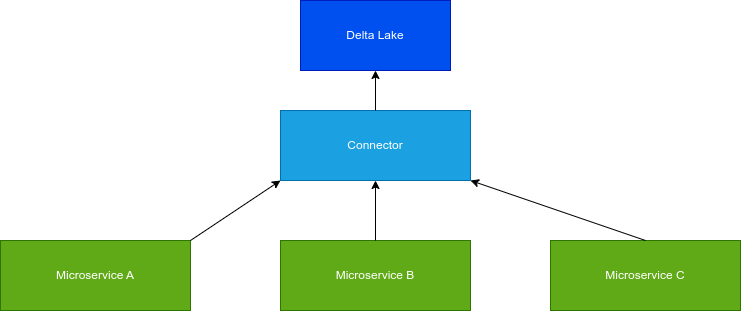
\includegraphics[width=\linewidth]{images/delta-lake-microservices.png}
\caption{Delta lake connectés à des microservices}\label{fig:schema-delta}
\end{figure}

\subsection{Partie Frontend}
Pour la mise en œuvre des microfrontends, Nous avons choisie d'utiliser principalement React pour les microfrontends, l'équipe de développement peut bénéficier de l'écosystème riche et mature de React, ainsi que de sa popularité croissante dans l'industrie du développement frontend. Cependant, il est également mentionné qu'Angular peut être utilisé ultérieurement si nécessaire, offrant ainsi une flexibilité supplémentaire dans le choix des technologies.

\begin{figure}[H]
\centering
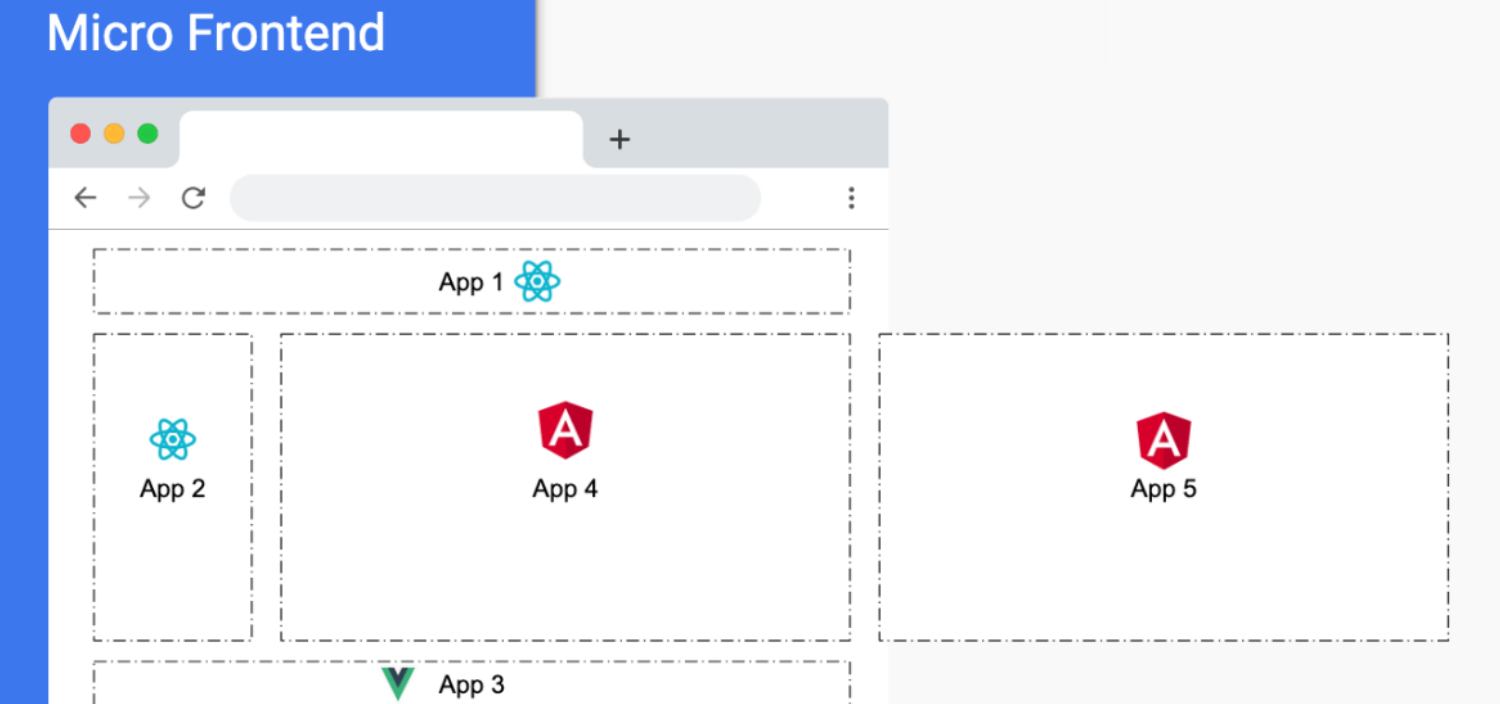
\includegraphics[width=\linewidth]{images/microfrontends.png}
\caption{Schéma des microfrontends}\label{fig:schema-microfrontends}
\end{figure}

\section*{Conclusion}
\addcontentsline{toc}{section}{Conclusion}
Lors de l'évaluation des différentes architectures de données pour Izicap, il est important de comprendre les besoins spécifiques liés à la gestion des fichiers bancaires, des reçus de transactions et des opérations d'agrégation.

Un data warehouse aurait pu être une option envisageable, offrant des structures de données organisées et optimisées pour les requêtes analytiques. Cependant, le principal inconvénient d'un data warehouse réside dans sa nature statique, qui nécessite une modélisation préalable des données et une transformation rigide avant leur chargement. Cela peut poser des défis lors de l'intégration de nouveaux types de fichiers ou de l'évolution des besoins en matière d'agrégation.

D'autre part, un data lake présente des avantages en termes de stockage économique et de flexibilité pour intégrer des données brutes et non structurées. Cependant, il peut être plus complexe de maintenir la qualité des données et la gouvernance, et des compétences techniques spécifiques sont nécessaires pour exploiter efficacement les données du data lake.

Donc, Delta Lake a été privilégié en raison de sa capacité à répondre aux besoins spécifiques d'Izicap en matière de gestion des fichiers bancaires, des reçus de transactions et des opérations d'agrégation. Il offre la flexibilité et la performance nécessaires tout en maintenant l'intégrité des données, ce qui en fait un choix solide pour l'architecture de données de l'entreprise.

En adoptant une approche basée sur les microservices, Izicap peut améliorer la flexibilité, la scalabilité et la maintenance de son application frontend. Cela permettra à l'entreprise de mieux répondre aux besoins changeants de ses utilisateurs, de faciliter la collaboration entre les équipes de développement et d'adopter des technologies innovantes pour offrir une expérience utilisateur optimale.

Les microfrontends offrent plusieurs avantages pour Izicap. Tout d'abord, la modularité inhérente aux microfrontends permet de développer, déployer et maintenir différentes parties de l'interface utilisateur de manière indépendante. Cela favorise la collaboration entre les équipes de développement et permet d'évoluer rapidement et efficacement. Chaque micro-application peut être développée en utilisant le framework et les technologies les plus adaptés à ses besoins spécifiques, ce qui offre une flexibilité technologique essentielle pour Izicap.

En revanche, l'approche monolithique présente des limitations en termes de scalabilité et de flexibilité technologique. Les modifications apportées à une partie de l'application peuvent avoir un impact sur l'ensemble du système, ce qui rend les évolutions plus complexes et risquées. De plus, l'introduction de nouvelles technologies ou frameworks peut être difficile dans une architecture monolithique, ce qui limite les possibilités d'innovation et de modernisation.


 
\chapter{--}\label{chap:3}
 \addcontentsline{toc}{section}{Introduction}

\section*{Introduction}
Dans ce chapitre, nous examinerons en détail les technologies clés qui sont utilisées dans notre solution pour fournir des fonctionnalités avancées et répondre aux besoins spécifiques de notre projet. Les trois principales technologies que nous aborderons sont Delta Lake, Trino et les Microfrontends.

\section{Delta Lake}

Delta Lake est une technologie de gestion des données qui permet de stocker, gérer et analyser des volumes massifs de données de manière efficace et fiable. Il repose sur une architecture basée sur des fichiers parquet et offre des fonctionnalités avancées telles que la gestion des transactions ACID (Atomicité, Cohérence, Isolation, Durabilité) et la compatibilité avec des outils d'analyse populaires. Delta Lake garantit également l'intégrité des données, la cohérence des requêtes et la prise en charge de la réplication et de la récupération en cas de défaillance.

Le concept de `lakehouse' est rendu possible grâce à Delta Lake. Il s'agit d'une architecture de données qui combine les avantages des entrepôts de données et des lacs de données, en offrant une approche unique et cohérente pour la gestion des données. Les données sont stockées au format Parquet dans le lac de données, permettant ainsi un traitement continu et par lots.
\begin{itemize}
    \item \textbf{Permet une architecture  Lakehouse:} Delta Lake permet une architecture de données continue et simplifiée qui permet aux organisations de gérer et de traiter d'énormes volumes de données en continu et par lots sans les tracas de gestion et d'exploitation liés à la gestion séparée du streaming, des data warehouses et des lacs de données.
    \item \textbf{Permet une gestion intelligente des données pour les lacs de données:} Delta Lake offre une gestion efficace et évolutive des métadonnées, qui fournit des informations sur les volumes de données massifs dans les lacs de données. Grâce à ces informations, les tâches de gouvernance et de gestion des données se déroulent plus efficacement.
    \item \textbf{Application du schéma pour une meilleure qualité des données:} Étant donné que les lacs de données n'ont pas de schéma défini, il devient facile pour les données mauvaises/incompatibles d'entrer dans les systèmes de données. La qualité des données est améliorée grâce à la validation automatique du schéma, qui valide la compatibilité DataFrame et table avant les écritures.
    \item \textbf{Permet la transaction ACID:} La plupart des architectures de données organisationnelles impliquent de nombreux mouvements ETL et ELT entrant et sortant du stockage de données, ce qui l'ouvre à plus de complexité et d'échecs aux points d'entrée des nœuds. Delta Lake garantit la durabilité et la persistance des données pendant l'ETL et d'autres opérations de données. Delta Lake capture toutes les modifications apportées aux données pendant les opérations de données dans un journal des transactions, garantissant ainsi l'intégrité et la fiabilité des données pendant les opérations de données.
\end{itemize}

\section{Principaux avantages et caractéristiques de Delta Lake}
\begin{flushleft}
	Avec Delta Lake, les données sont stockées dans un format optimisé, tel que Parquet, dans un lac de données. Ce format facilite le traitement efficace des requêtes, quel que soit le mode d'accès aux données, qu'il s'agisse d'un traitement streaming ou par batch.
\end{flushleft}

\begin{figure}[H]
\centering
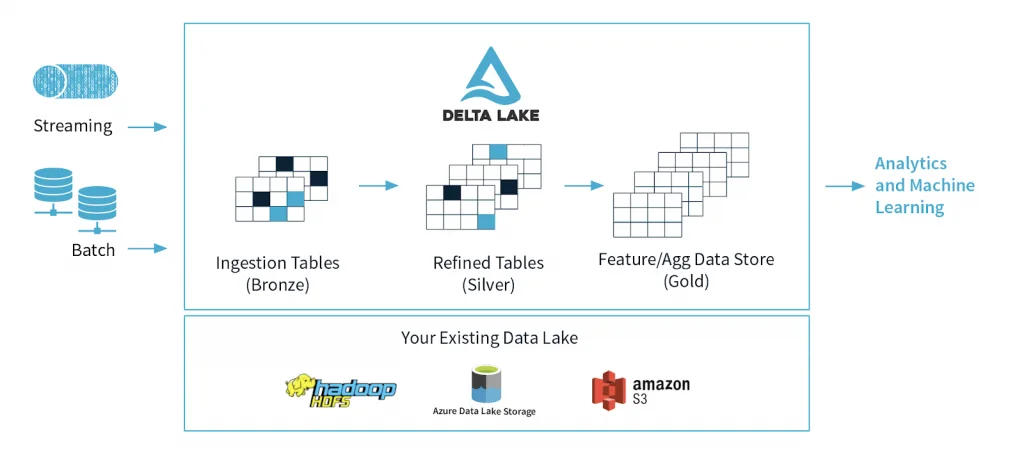
\includegraphics[width=\linewidth]{images/delta_lake_architecture.png}
\caption{Architecture multi-sauts de Delta Lake}\label{fig:delta-lake-architecture}
\end{figure}

\begin{itemize}
	\item[\textbullet] \textbf{Pistes d'audit et historique:}Dans Delta Lake, chaque écriture existe en tant que transaction et est enregistrée en série dans un journal des transactions. Par conséquent, toutes les modifications ou validations apportées au journal des transactions sont enregistrées, laissant une trace complète à utiliser dans les audits historiques, la gestion des versions ou à des fins de voyage dans le temps. Cette fonctionnalité de Delta Lake permet de garantir l'intégrité et la fiabilité des données pour les opérations de données d'entreprise.
	\item[\textbullet] \textbf{Voyager dans le temps et versionner les données:} Étant donné que chaque écriture crée une nouvelle version et stocke l'ancienne version dans le journal des transactions, les utilisateurs peuvent afficher/restaurer les anciennes versions de données en fournissant l'horodatage ou le numéro de version d'une table ou d'un répertoire existant à l'API de lecture Sparks\@. À l'aide du numéro de version fourni, Delta Lake construit ensuite un instantané complet de la version avec les informations fournies par le journal des transactions. Les retours en arrière et la gestion des versions jouent un rôle essentiel dans l'expérimentation de l'apprentissage automatique, où les scientifiques des données modifient de manière itérative les hyperparamètres pour former des modèles et peuvent revenir aux modifications si nécessaire.
	\item[\textbullet] \textbf{Unifie le traitement par lots et par flux:} Chaque table d'un Delta Lake est un puits de lot et de flux. Avec le streaming structuré Sparks, les organisations peuvent diffuser et traiter efficacement les données de streaming. De plus, grâce à la gestion efficace des métadonnées, à la facilité d'évolutivité et à la qualité ACID de chaque transaction, l'analyse en temps quasi réel devient possible sans utiliser une architecture de données à deux niveaux plus compliquée.
	\item[\textbullet] \textbf{Gestion efficace et évolutive des métadonnées:} Delta Lakes stocke les informations de métadonnées dans le journal des transactions et exploite la puissance de traitement distribuée de Spark pour traiter rapidement, lire et gérer efficacement de gros volumes de métadonnées de données, améliorant ainsi la gouvernance des données.
	\item[\textbullet] \textbf{transactions ACID:} Delta Lakes garantit que les utilisateurs voient toujours une vue de données cohérente dans une table ou un répertoire. Il garantit cela en capturant chaque modification effectuée dans un journal de transactions et en l'isolant au niveau d'isolation le plus fort, le niveau sérialisable. Au niveau sérialisable, chaque opération existante a et suit une séquence en série qui, lorsqu'elle est exécutée une par une, fournit le même résultat que celui indiqué dans le tableau.
	\item[\textbullet] \textbf{Opérations du langage de manipulation de données:} Delta Lakes prend en charge les opérations DML telles que les mises à jour, les suppressions et les fusions, qui jouent un rôle dans les opérations de données complexes telles que la capture de données de modification (CDC), les upserts en continu et la dimension à évolution lente (SCD). Des opérations comme CDC assurent la synchronisation des données dans tous les systèmes de données et minimisent le temps et les ressources consacrés aux opérations ELT. Par exemple, en utilisant le CDC, au lieu d'ETL toutes les données disponibles, seules les données récemment mises à jour depuis la dernière opération subissent une transformation.
	\item[\textbullet] \textbf{Schema Enforcement:} Delta Lakes effectue une validation automatique du schéma en vérifiant un ensemble de règles pour déterminer la compatibilité d'une écriture d'un DataFrame vers une table. L'une de ces règles est l'existence de toutes les colonnes DataFrame dans la table cible. Une occurrence d'une colonne supplémentaire ou manquante dans le DataFrame génère une erreur d'exception. Une autre règle est que le DataFrame et la table cible doivent contenir les mêmes types de colonnes, ce qui, sinon, déclenchera une exception. Delta Lake utilise également DDL (Data Definition Language) pour ajouter explicitement de nouvelles colonnes. Cette fonctionnalité de lac de données permet d'éviter l'ingestion de données incorrectes, garantissant ainsi une qualité élevée des données.
	\item[\textbullet] \textbf{Compatibilité avec l'API de Spark:} Delta Lake est basé sur Apache Spark et est entièrement compatible avec l'API Spark, qui permet de créer des pipelines de données volumineuses efficaces et fiables.
	\item[\textbullet] \textbf{Flexibilité et intégration:} Delta Lake est une couche de stockage open source et utilise le format Parquet pour stocker des fichiers de données, ce qui favorise le partage de données et facilite l'intégration avec d'autres technologies et stimule l'innovation.
\end{itemize}

\section{Trino}

Trino, anciennement connu sous le nom de Presto, est un moteur de requêtes SQL distribué et open-source. Il est conçu pour exécuter des requêtes interactives et analytiques à grande échelle sur des données hétérogènes et distribuées. Trino offre une grande polyvalence en permettant l'accès à différents types de sources de données, qu'il s'agisse de bases de données relationnelles, de systèmes de fichiers, de sources de données en temps réel ou de services de stockage cloud. Grâce à sa conception distribuée, Trino permet des performances élevées et une scalabilité horizontale, ce qui en fait un outil essentiel pour l'analyse des données dans notre solution.

\begin{figure}[H]
\centering
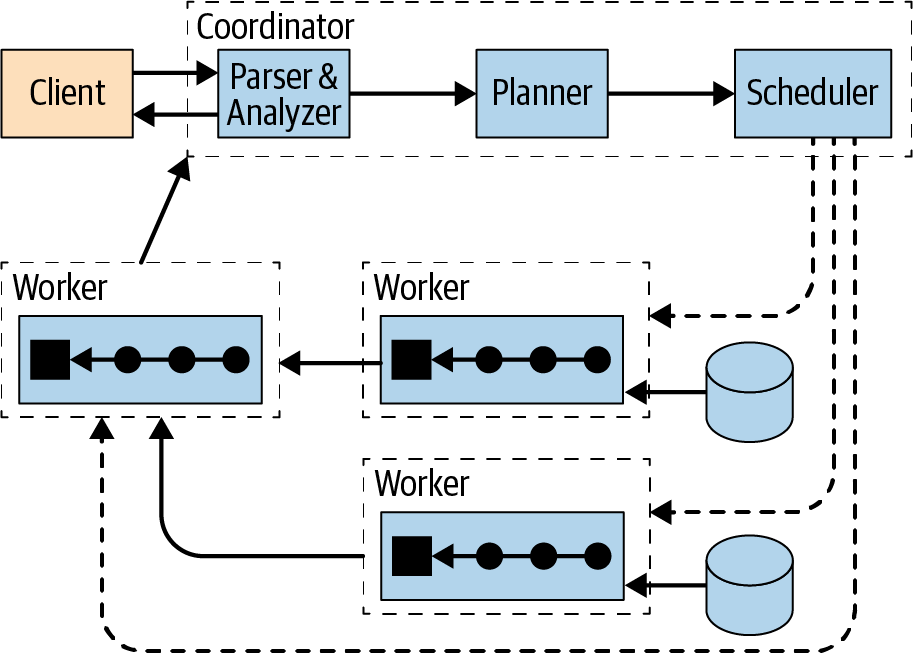
\includegraphics[width=0.8\linewidth]{images/trino_architecture.png}
\caption{Vue d'ensemble de l'architecture Trino avec le coordinateur et les workers}\label{fig:trino-architecture}
\end{figure}

\begin{enumerate}
	\item Un coordinateur est un serveur Trino qui gère les requêtes entrantes et gère les workers pour exécuter les requêtes.
	\item Un worker est un serveur Trino responsable de l'exécution des tâches et du traitement des données.
	\item Le service de découverte s'exécute généralement sur le coordinateur et permet aux workers de s'inscrire pour participer au cluster.
	\item Toutes les communications et tous les transferts de données entre les clients, le coordinateur et les workers utilisent des interactions basées sur REST sur HTTP/HTTPS.
\end{enumerate}

\section{Springboot}

Spring Boot est un framework open-source pour le développement d'applications Java. Il fournit une approche simplifiée et conventionnelle pour créer des applications Java autonomes, prêtes à être déployées, sans nécessiter une configuration complexe.

L'un des principaux avantages de Spring Boot est sa capacité à réduire la configuration boilerplate et à simplifier le développement d'applications en fournissant des définitions de configuration par défaut intelligentes et en automatisant de nombreux aspects du développement. Il intègre également un serveur d'applications embarqué, ce qui facilite le déploiement et l'exécution de l'application sans avoir besoin d'un serveur d'applications externe.

Spring Boot suit le paradigme de la programmation orientée annotation, où les annotations sont utilisées pour configurer et orchestrer les différentes parties de l'application. Il offre une large gamme de fonctionnalités, telles que l'injection de dépendances, la configuration externe, la gestion des erreurs, la sécurité, l'accès aux données, etc. Ces fonctionnalités sont regroupées dans des starters, qui sont des dépendances prédéfinies facilitant l'ajout de fonctionnalités spécifiques à l'application.

Grâce à son approche simplifiée, Spring Boot permet aux développeurs de se concentrer davantage sur la logique métier de leur application plutôt que sur des tâches de configuration fastidieuses. Il favorise également les bonnes pratiques de développement, telles que la séparation des préoccupations et la modularité, ce qui rend les applications plus maintenables et évolutives.


\section{Keycloak}

Keycloak est une solution open-source de gestion des identités et des accès (Identity and Access Management) développée par Red Hat. Il fournit des fonctionnalités complètes pour la gestion des utilisateurs, l'authentification, l'autorisation et la sécurisation des applications.

Keycloak permet de centraliser et de simplifier la gestion des identités au sein d'une infrastructure informatique. Il offre des fonctionnalités telles que l'inscription des utilisateurs, l'authentification à plusieurs facteurs, la gestion des rôles et des autorisations, la gestion des sessions, ainsi que l'intégration avec des protocoles d'authentification et d'autorisation courants tels que OAuth 2.0 et OpenID Connect.

Keycloak offre un ensemble de fonctionnalités pour gérer les rôles, les administrateurs, les utilisateurs et les mots de passe. Voici comment Keycloak aborde ces aspects:

\begin{enumerate}
	\item Keycloak permet de définir des rôles au niveau du royaume (realm) ou au niveau de l'application. Les rôles peuvent être créés et attribués aux utilisateurs pour définir leurs autorisations et leurs accès.
	\item Les administrateurs Keycloak peuvent créer, gérer et assigner des rôles aux utilisateurs via l'interface d'administration ou via l'API de gestion.
	\item Les rôles peuvent être utilisés pour contrôler l'accès aux fonctionnalités, aux pages et aux ressources au sein de l'application.
	\item Keycloak propose des rôles d'administration spécifiques tels que "admin" ou "superadmin" qui permettent aux utilisateurs d'effectuer des tâches d'administration, telles que la gestion des clients, des utilisateurs, des rôles, etc.
	\item Les utilisateurs peuvent se connecter à l'aide de leurs identifiants (nom d'utilisateur et mot de passe) ou d'autres méthodes d'authentification prises en charge, telles que l'authentification à deux facteurs, OAuth 2.0, etc.
	\item Keycloak prend en charge l'authentification basée sur les utilisateurs et fournit une interface d'inscription pour permettre aux utilisateurs de créer leurs comptes.
	\item Keycloak offre également des fonctionnalités d'authentification avancées, telles que l'authentification à deux facteurs, l'authentification sociale (via des fournisseurs d'identité tels que Google, Facebook, etc.) et l'authentification basée sur des certificats.
\end{enumerate}

\section{Kafka}

Kafka est une plateforme de streaming de données distribuée et évolutive, conçue pour gérer efficacement la transmission et le traitement de flux de données en temps réel. Elle a été développée par Apache Software Foundation.

Kafka est basé sur une architecture de journal de messages distribué, où les données sont stockées sous forme de flux de messages dans des "topics". Les producteurs de données envoient des messages à des "topics" spécifiques, tandis que les consommateurs s'abonnent à ces "topics" pour récupérer les messages. Cela permet une communication asynchrone et une séparation claire entre les producteurs et les consommateurs de données.

Les principales caractéristiques de Kafka incluent:

\begin{enumerate}
	\item Scalabilité: Kafka est conçu pour gérer de gros volumes de données et peut être mis à l'échelle horizontalement pour répondre aux besoins de performance croissants. Il peut gérer des charges de travail élevées et traiter des milliers de messages par seconde.
	\item Tolérance aux pannes: Kafka garantit une haute disponibilité et une tolérance aux pannes en répliquant les données sur plusieurs nœuds du cluster. Cela garantit la fiabilité et la disponibilité des données, même en cas de défaillance d'un ou plusieurs nœuds.
	\item Durabilité des données: Les messages stockés dans Kafka sont persistants et peuvent être conservés pendant une période définie. Cela permet de rejouer les messages et de récupérer les données en cas de besoin, ce qui est essentiel pour les cas d'utilisation nécessitant une conservation à long terme des données.
	\item Traitement de flux: Kafka est conçu pour le traitement de flux en temps réel. Il permet aux applications de consommer des flux de données en continu et de les traiter en temps réel, ce qui est crucial pour les cas d'utilisation nécessitant une analyse en temps réel, des pipelines de données, etc.
	\item Intégration avec d'autres outils: Kafka s'intègre facilement avec d'autres outils et frameworks tels que Spark, Hadoop, Flink, etc. Cela permet une intégration transparente avec l'écosystème Big Data et facilite l'ingestion, le traitement et la diffusion des données.
\end{enumerate}

\begin{figure}[H]
\centering
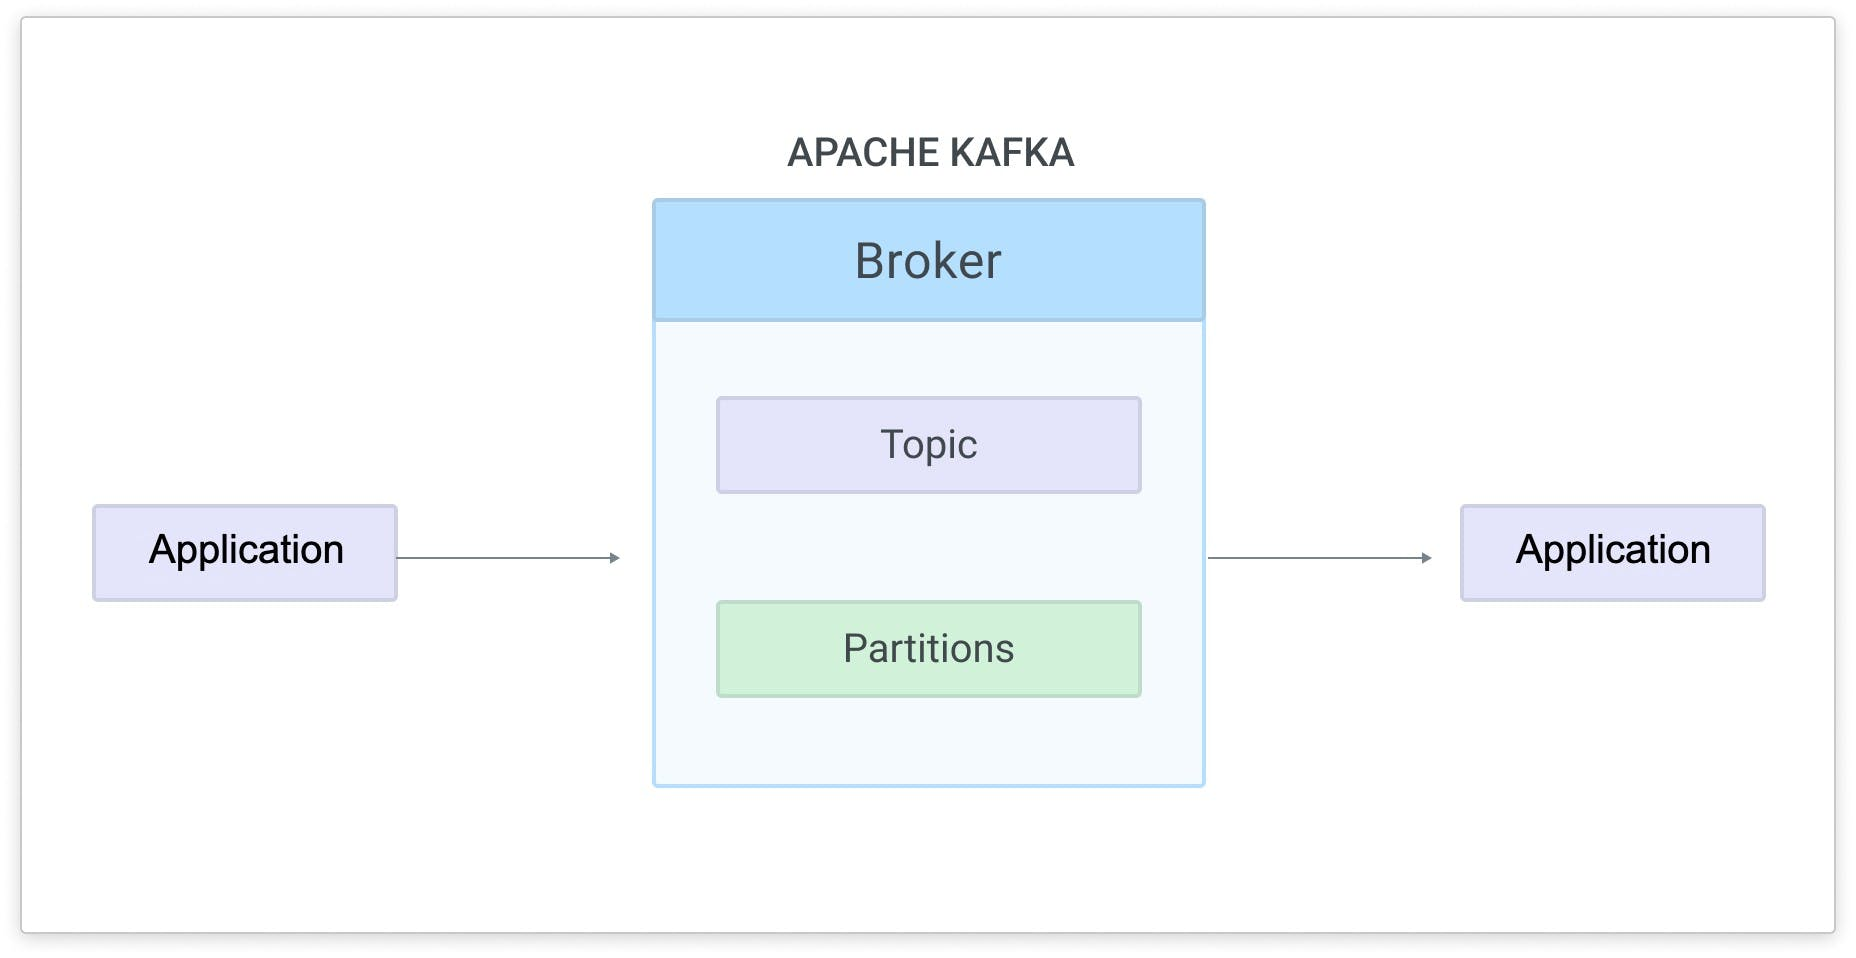
\includegraphics[width=\linewidth]{images/kafka.jpg}
\caption{Architecture Kafka}\label{fig:kafka}
\end{figure}

 
% \include{perspectives}
%%conclusion
\conclusion
Le stage a été une expérience enrichissante qui a permis d'explorer divers aspects des microservices en utilisant des technologies telles que Delta Lake, Trino, Spring Boot, et Keycloak. L'environnement de travail était propice à l'apprentissage et à la mise en pratique de ces concepts.

L'adoption des microservices présente de nombreux avantages par rapport à une architecture monolithique. Les microservices offrent une meilleure scalabilité et flexibilité, permettant le déploiement, le développement et la mise à l'échelle indépendants de chaque service. De plus, la communication entre les microservices via des API facilite l'intégration et la collaboration entre les différentes parties du système.

Pendant le stage, nous avons appris à concevoir et implémenter des microservices en utilisant Spring Boot, en exploitant ses fonctionnalités de persistence, de sécurité, et de création d'API REST. Nous avons également intégré Keycloak pour gérer l'authentification et l'autorisation des utilisateurs dans notre architecture de microservices. L'utilisation de Delta Lake a permis de garantir la fiabilité des données et de faciliter la gestion des mises à jour.
% 
\lhead[]{} \rhead[]{} \chead[]{}

%%biblio
\addcontentsline{toc}{chapter}{Bibliographie}
\bibliographystyle{abbrv}
\bibliography{biblio}


%\chapter*{Annexe}\addcontentsline{toc}{chapter}{Annexe}\label{annexe1}

\subsection*{Étapes clés du déroulement de l'attaque}


Nous allons exploiter quelques failles de ce réseau pour effectuer une attaque man in the middle (MITM).\\

Au début, notre machine Windows peut atteindre normalement le routeur R4.
\begin{figure}[H]
    \centering
    \includegraphics[scale=0.8]{images/ping_b4_1}
    \caption{Ping vers le routeur R4 avec succès}
    \label{fig:ping_b4_1}
\end{figure}
Quand on essaie de tracer le chemin vers R4, on constate que la machine passe par le routeur R1 légitime du lien pour atteindre R4
\begin{figure}[H]
    \centering
    \includegraphics{images/tracert_b4_1}
    \caption{Traces du chemin vers R4}
    \label{fig:tracert_b41}
\end{figure}
L'attaquant sur le lien peut alors passer a l'attaque.
Pour effectuer l'attaque MITM on utilisera l'outil fake\_router6, un utilitaire du package d'outils \textbf{the hacker choice}.
Ainsi sur la machine d'attaque, on active en un premier lieu le forwarding pour être transparent et ne pas bloquer le transit des paquets.
\begin{figure}[H]
    \centering
    \includegraphics{images/attk/fwrd_activation}
    \caption{Activation du forwarding des paquets.}
    \label{fig:activ_fwrd}
\end{figure}
Aussi on lance wireshark pour observer le trafic des paquets sur notre interface dans le réseau.\\
-------\\
Puisque tout est prêt nous allons lancer l'attaque.

\begin{figure}[H]
    \centering
    \includegraphics[scale=0.8]{images/attk/lancement_attk_1}
    \caption{Initialisation de l'attaque}
    \label{fig:attk_init_1}
\end{figure}

L'attaque est en cours et l'attaquant s'annonce comme le routeur par défaut du lien
nous allons maintenant vérifier la table des routes de notre machine windows.
\begin{figure}[H]
    \centering
    \includegraphics{images/attk/tableRoutes_windows}
    \caption{Table des routes de la machine victime}
    \label{fig:win_route_table}
\end{figure}
On constate que l'attaquant s'est insère comme passerelle de la victime.
pour confirmer cela reprenons un tracert vers le routeur r4
\begin{figure}[H]
    \centering
    \includegraphics{images/attk/tracert_b4_2}
    \caption{Chemin vers b4 pendant l'attaque.}
    \label{fig:tracert_b42}
\end{figure}
On peut voir clairement que la victime passe par l'attaquant pour atteindre le routeur.\\

A présent nous allons essayer de capturer une information envoyée par la victime.
Pour cela la victime fait un telnet sur le router R4 pour s'y connecter avec les paramètres suivants:\\
password1:\textbf{cisco}\\
password2:\textbf{class}
\begin{figure}[H]
    \centering
    \includegraphics{images/attk/telnet_r4}
    \caption{Connexion telnet au routeur.}
    \label{fig:telnetr4}
\end{figure}

Une fois la connexion réussie, nous allons voir avec wireshark les paquets de connexion et y retrouver les paramètres de connexion.
\begin{figure}[H]
    \centering
    \includegraphics[width=1.0\textwidth]{images/attk/c}
    \includegraphics[width=1.0\textwidth]{images/attk/i}
    \includegraphics[width=1.0\textwidth]{images/attk/s}
    \includegraphics[width=1.0\textwidth]{images/attk/c2}
    \includegraphics[width=1.0\textwidth]{images/attk/o}   
    \caption{Premier paramètre de connexion au routeur R4: \textbf{c-i-s-c-o}}
    \label{fig:param_conn_r4}
\end{figure}
\begin{figure}[H]
    \centering
    \includegraphics[width=1.0\textwidth]{images/attk/param2_c}
    \includegraphics[width=1.0\textwidth]{images/attk/param2_l}
    \includegraphics[width=1.0\textwidth]{images/attk/param2_a}
    \includegraphics[width=1.0\textwidth]{images/attk/param2_s1}
    \includegraphics[width=1.0\textwidth]{images/attk/param2_s2}
    \caption{Second paramètre de connexion au routeur R4: \textbf{c-l-a-s-s}}
    \label{fig:param_conn2}
\end{figure}
Les paramètres on été retrouves donc l'attaque a été un succès!

%\subsection*{Mitigations}
%Pour sécuriser ce réseau afin d'éviter ce genre d'attaque, deux mesures de sécurité peuvent être configurées.
%\begin{itemize}
%    \item le SEND
%    \item le RaGuard
%\end{itemize}





\end{document}          
